\documentclass[tikz, border=1pt]{standalone}
\pdfoutput=1 % if your are submitting a pdflatex (i.e. if you have
             % images in pdf, png or jpg format)

\usepackage{graphicx}

% Use the tikz package
\usepackage{tikz}
\usetikzlibrary{decorations}


\begin{document}

        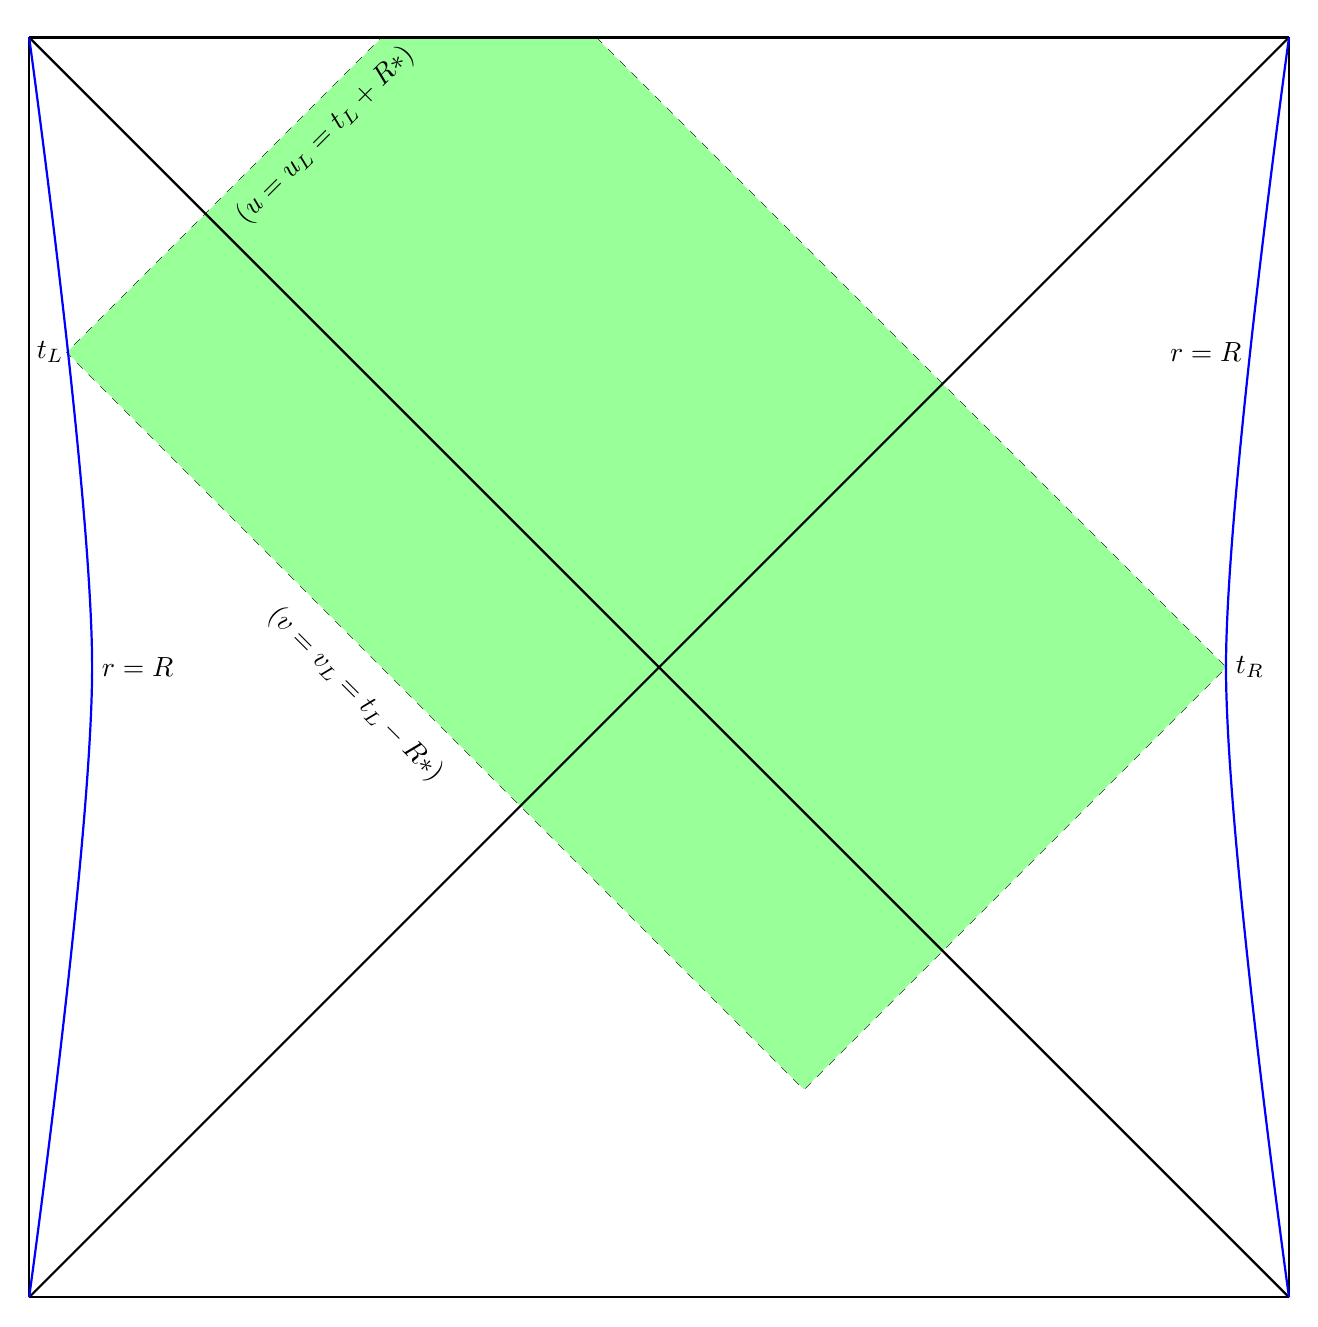
\begin{tikzpicture}[scale=4]
        
        % WdW boundaries
        \draw[dashed] (1.8,4)--(3.8,2)--(2.46,0.66)--(0.12,3)--(1.12,4)--(2,4); 
        \fill[green!40!white] (1.8,4)--(3.8,2)--(2.46,0.66)--(0.12,3)--(1.12,4)--(2,4) ;
        
        %axes
        \draw[thick] (0,0)--(4,0);
        \draw[thick] (4,0) --(4,4);
        \draw[thick] (4,4)--(0,4);
        \draw[thick] (0,4)--(0,0);
        \draw[thick] (0,0) --(4,4);
        \draw[thick] (0,4)--(4,0);
        
        % cutoff
        \draw[blue,thick] plot [smooth] coordinates {(0,0) (0.2,2) (0,4)};
        \draw[blue,thick] plot [smooth] coordinates {(4,0) (3.8,2) (4,4)};
        
        %labels
        \draw (0.14,3) node[left]{$t_L$};
        \draw (3.8,2) node[right]{$t_R$};
        \draw (0.2,2) node[right] {$r=R$};
        \draw (3.88,3) node[left] {$r=R$};
        \draw (.75,2.2) node[right, rotate=-45]{$(v=v_L=t_L-R*)$};
        \draw (.65,3.4) node[right, rotate=45]{$(u=u_L=t_L + R*)$};
        \end{tikzpicture}

\end{document}
